% ============================================================
% §4  Experiments
% ============================================================

\section{Experiments}
\label{sec:experiments}

\subsection{Experimental Setup}
\label{sec:setup}

\subsubsection{Datasets and Benchmark Protocol}
\label{sec:datasets}

\paragraph{Datasets.}
We evaluate CSMAD on six real-world multivariate benchmark families --- SWaT~\cite{goh2016swat},
WaDi~\cite{ahmed2017wadi}, PSM~\cite{abdulaal2021psm}, SMD~\cite{su2019omnianomaly}, SMAP, and
MSL~\cite{hundman2018telemanom} --- spanning industrial control, IT infrastructure, and spacecraft
telemetry: 113 entities in total, or 114 evaluation conditions with SWaT's dual evaluation
(detailed below).
Table~\ref{tab:datasets} summarizes per-family statistics; per-entity detail is in
\ref{sec:appendix_dataset}.

% ---- Table 1: Dataset statistics ----
%% PDF QA r1 BLOCKER-1/BLOCKER-A: was a single-column \begin{table} whose natural
%% width exceeded the column/text width in both builds (right-edge truncation).
%% D-013 (prose/space compression): cell + header abbreviation (SWaT dual condition
%% folded to a dagger defined in the caption; "(\%)" moved into the caption) lets
%% the table return to a single-column float, reclaiming the r2 full-width
%% table* band (~0.1p).  \scriptsize + \tabcolsep 2pt + max-width cap.
\begin{table}[t]
\scriptsize
\centering
\caption{Dataset statistics under the contaminated benchmark protocol, summarized per family.
  Train/test sizes reflect the re-split described in \S\ref{sec:datasets}.
  Train AR = anomaly ratio (\%) in the training portion (originating from the incorporated
  test prefix); Test AR = anomaly ratio (\%) in the held-out evaluation portion.
  The WaDi row aggregates the two independent entities A1/A2 (values given as A1\,/\,A2);
  SMD, SMAP, and MSL values are per-entity averages or concatenated totals as indicated.
  SWaT is evaluated under both full and excl22 conditions ($\dagger$: full\,/\,excl22);
  Table~\ref{tab:main_results} uses excl22 (\S\ref{sec:datasets}).
  Per-entity statistics are in \ref{sec:appendix_dataset} (Table~\ref{tab:per_entity}).}
\label{tab:datasets}
\setlength{\tabcolsep}{2pt}
\begin{adjustbox}{max width=\linewidth}
\begin{tabular}{lrrrcc@{}}
\toprule
Family & \#Train & \#Test & \#Dim. & Train AR & Test AR \\
\midrule
SWaT (A1+A2) & 719{,}959 & 224{,}960 & 45 & 1.63 & 19.05\,/\,3.68$^{\dagger}$ \\
WaDi (A1\,/\,A2) & 1{,}296{,}001\,/\,870{,}972 & 86{,}401\,/\,86{,}402 & 123 & 0.52\,/\,0.76 & 3.82\,/\,3.87 \\
PSM & 176{,}401 & 43{,}921 & 25 & 6.20 & 30.63 \\
SMD ($\times$28) & \multicolumn{2}{c}{per-machine (\S A.3)} & 29--36 & per-machine & [X.XX] (avg, pending) \\
% PH:NUM-032 | SMD held-out-suffix Test AR, 28-machine average (re-split, per-machine pending)
SMAP ($\times$54) & 355{,}905 & 217{,}925 & 25 & 0.70 & 24.54 \\
MSL ($\times$27) & 95{,}271 & 36{,}775 & 55 & 1.70 & 16.72 \\
\bottomrule
\end{tabular}
\end{adjustbox}
\end{table}

\paragraph{Contaminated benchmark protocol.}
A defining feature of standard MTSAD benchmarks is that their original training splits contain
no labeled anomalies by construction~\cite{goh2016swat,ahmed2017wadi,abdulaal2021psm,%
su2019omnianomaly,hundman2018telemanom} (per-family label semantics in
\ref{sec:appendix_dataset}), so a method that exploits labeled anomalies cannot be
evaluated without modifying the partition.
We therefore re-split each dataset at the temporal midpoint of its original test file: the earlier
half is appended to the training data and the later half is reserved exclusively for evaluation,
so labeled anomalies are present in training.
Training anomaly ratios range from 0.52\% to 6.20\% (SMD per-machine values pending;
Table~\ref{tab:datasets}).
The evaluation half is never observed during training or threshold selection, so no temporal
lookahead is introduced and no model sees evaluation labels at any stage; the identical partition
is applied to all methods (Section~\ref{sec:baselines}).
The halving rule is uniform; only for SMAP/MSL does the split point shift when it falls within
ten timesteps of an annotated anomaly region (4 of 81 channels are affected; largest shift:
166 timesteps; \ref{sec:appendix_dataset}).
This practice has precedent: NRdetector~\cite{wang2025nrdetector} likewise re-splits standard
benchmarks (at a 7:3 ratio) so that anomalous events fall within the training stream.
One limitation remains: the anomaly type distribution of the incorporated prefix may differ from
that of the evaluation suffix.
Inputs are min--max scaled per feature on each entity's training portion, multi-entity families
normalized per entity.

\paragraph{SWaT dual evaluation.}
SWaT is trained once but evaluated twice: in the full condition, a single attack event (region~22)
accounts for 83.75\% of test anomaly mass, so the full metric chiefly reflects this one event.
We therefore also report all metrics with region~22 masked out, denoted excl22
(anomaly ratio 3.68\% versus 19.05\%): the model and scores are identical, only the evaluation
mask differs, applied identically to all baselines.
Table~\ref{tab:main_results} ranks methods under the excl22 condition; the region-22 derivation
and full-condition results are in \ref{sec:appendix_swat}.

\subsubsection{Implementation Details}
\label{sec:impl}

\paragraph{Architecture and training.}
CSMAD uses patch size 10 on windows of length 500 (masking ratio 0.15), a 4-layer encoder
($d_{\mathrm{model}}=512$, fixed across entities), and a 3-layer Teacher with a 2-layer Student
decoder; training runs 500 epochs (Teacher-only for the first 250; Section~\ref{sec:decoders})
at batch size 1024, one seed-42 run per entity.
We report no cross-seed variance or confidence intervals for the main results, a limitation of
the current evaluation, except for the random-score baseline, which is averaged over five runs
(\ref{sec:appendix_impl}).
Full hyperparameters, environment, and preprocessing are in
\ref{sec:appendix_impl} and~\ref{sec:appendix_dimensionality}.

\paragraph{Epoch asymmetry disclosure.}
Unsupervised baselines train for 10 epochs and weakly supervised baselines for 50 epochs, both
evaluated every epoch; CSMAD trains for 500 epochs, evaluated every 5 (full budget table in
\ref{sec:appendix_impl}).
All methods share the same selection criterion, run to their full budget without early stopping,
and are reported at their best evaluated epoch.
Budget differences reflect each method's convergence characteristics: CSMAD requires the
250-epoch warmup before the Student activates; baseline batch sizes follow each method's original
preset (Table~\ref{tab:baseline_hparams} in \ref{sec:appendix_impl}).
We report this asymmetry transparently; \ref{sec:epoch_sensitivity} analyzes
epoch-budget sensitivity for representative baselines.

\paragraph{Test-set model selection.}
Best-epoch selection for CSMAD and all 26 baselines evaluates PA\%K-AUC F1 on the test split,
as no separate validation split exists in this protocol.
Because the criterion is applied uniformly to all methods, relative rankings are unaffected;
however, absolute estimates may be optimistically biased, and we acknowledge this limitation.

\paragraph{Inference and threshold.}
Inference uses the leave-one-out masking of Section~\ref{sec:scoring} (wall-clock cost in
\ref{sec:cost}).
Threshold-dependent metrics use the anomaly-ratio threshold: the $(1-\alpha)$ quantile of the
score distribution, where $\alpha$ is the measured anomaly fraction of the evaluation span.
This threshold is applied identically to all methods and follows the anomaly-ratio thresholding
of~\cite{xu2022anomalytransformer}; our $\alpha$ derives from evaluation-set ground truth but is
never used in training.
Threshold-free metrics (VUS, PA\%K-AUC families) are unaffected.

\subsubsection{Evaluation Metrics}
\label{sec:metrics}

We adopt five metrics that assess complementary aspects of detection quality, following the
multi-metric philosophy of recent benchmark
analyses~\cite{kim2022rigorous,paparrizos2022vus,liu2024elephant,wang2025nrdetector}.
\textbf{PA\%K-AUC F1} integrates the point-adjusted F1 of the PA\%K
protocol~\cite{kim2022rigorous} over the tolerance spectrum $K \in \{0,1,\ldots,100\}$,
eliminating sensitivity to the choice of $K$; it is our primary metric and selection criterion.
\textbf{PA\%K-AUC AUC-PR} applies the same $K$-integration to the area under the
precision--recall curve, complementary under class imbalance.
\textbf{VUS-PR} and \textbf{VUS-ROC}~\cite{paparrizos2022vus} sweep both a decision threshold
and a temporal tolerance to measure ranking quality without a fixed operating point; VUS-PR was
identified as the most reliable single measure for time-series anomaly detection by a large-scale
study~\cite{liu2024elephant}.
\textbf{Affiliation F1}~\cite{huet2022affiliation} is the harmonic mean of affiliation precision
and recall, quantifying the temporal proximity between predicted and ground-truth events; it is
computed at the anomaly-ratio threshold (the F1-optimal-threshold variant is excluded from all
rankings).
Formal definitions are in \ref{sec:appendix_metrics}.

The five metrics span three orthogonal perspectives: threshold-free ranking (VUS),
tolerance-spectrum integration (PA\%K-AUC), and local event localization (Affiliation F1).
Each perspective has distinct failure modes; reporting all five prevents any single failure mode
from going undetected.
The traditional point-adjusted F1 (PA F1) at $K{=}0$~\cite{xu2018kpivae} is reported only in
\ref{sec:appendix_full_results} for comparability with prior work, labeled (oracle) to
indicate that its threshold is selected to maximize F1, and is never used for ranking: even a
random score can reach state-of-the-art levels under it~\cite{kim2022rigorous}.

\subsubsection{Baselines and Comparison Conditions}
\label{sec:baselines}

We compare against 26 baselines: 22 unsupervised and four weakly supervised.
The unsupervised group comprises nine simple or lightweight detectors following~\cite{sarfraz2024quovadis}, six established deep MTSAD systems~\cite{xu2022anomalytransformer,tuli2022tranad,audibert2020usad,zong2018dagmm,deng2021gdn,su2019omnianomaly}, and seven recent competitive methods, including TFMAE (Section~\ref{sec:related_mae})~\cite{fang2024tfmae,lai2023npsr,wu2023timesnet,yang2023dcdetector,song2023memto,luo2024moderntcn,wu2025catch}.
The four weakly supervised methods exploit labeled anomalies during training~\cite{sultani2018deepmil,lee2021wetas,liu2024treemil,wang2025nrdetector}; the full tier list, implementation provenance (including the simplified DAGMM variant), and hyperparameters are in \ref{sec:appendix_impl}.
The weakly supervised group is evaluated under the contaminated-training condition only (defined below), since the anomaly-excised condition removes all labeled anomalies and would eliminate the positive windows their objectives require.

\paragraph{Comparison conditions.}
The main comparison uses the \textbf{anomaly-excised condition} for all 22 unsupervised
baselines: labeled anomaly regions are excised from the contaminated training data, and the
surviving normal segments are concatenated with boundary-aware windowing.
Under a purely unsupervised objective a labeled anomaly can be used only negatively, as a
contaminating sample to remove; the anomaly-excised condition grants each unsupervised method this
most favorable use of the labels, while CSMAD trains on the full contaminated set.
Excision reduces baseline training volume by the train anomaly ratio (0.52\%--6.20\%; SMD
pending), which may itself contribute to the gap; the protocol-effect block of
Table~\ref{tab:main_results} decouples these effects, and \ref{sec:contaminated_results} reports
the complementary \textbf{contaminated-training condition} (full stream, no excision) for all
unsupervised baselines.

\subsection{Main Results}
\label{sec:main_results}

Table~\ref{tab:main_results} presents PA\%K-AUC F1 and VUS-PR for CSMAD and all 26 baselines
across the six dataset families; full five-metric and per-entity results are in
\ref{sec:appendix_full_results} and \ref{sec:appendix_entity_results}.

% ---- Table 2: Main results ----
%% PDF QA r1 BLOCKER-2/MAJOR-6 + fallback ladder (a): sidewaystable broke the
%% twocolumn build (column-float overprint) and was over-wide even rotated in
%% preprint.  Converted to an upright two-column table* with \scriptsize,
%% \tabcolsep 2pt, and a max-width cap (recovers ~0.4p vs a rotated float page).
\begin{table*}[t]
\scriptsize
\centering
\caption{Main comparison results under the contaminated benchmark protocol
  (anomaly-excised condition for unsupervised baselines; contaminated-training condition for
  weakly supervised baselines; \S\ref{sec:baselines}).
  Reported metrics: PA\%K-AUC F1 and VUS-PR; the remaining three metrics are in
  \ref{sec:appendix_full_results}.
  SWaT column uses the excl22 evaluation condition; full-condition results appear in
  \ref{sec:appendix_swat}.
  SMD, SMAP, and MSL values are macro-averages over all entities (per-entity results in
  \ref{sec:appendix_entity_results}).
  \textbf{Bold} = highest; \underline{underline} = second-highest.
  \textit{Bottom block (protocol effect, \S\ref{sec:main_results})}: CSMAD and [N]
  representative unsupervised baselines under a standard clean-train split (original training
  file only, no labeled anomalies), evaluated on the identical held-out evaluation suffix;
  standard-split CSMAD uses the identical configuration with all label-dependent paths
  automatically inactive in the absence of positive training windows.
  Cells are populated only for the representative protocol-effect dataset columns.}
  % PH:NUM-014 | number of representative baselines in protocol-effect block
\label{tab:main_results}
\setlength{\tabcolsep}{2pt}
\begin{adjustbox}{max width=\linewidth}
\begin{tabular}{l@{\hspace{4pt}}l@{\hspace{3pt}}cccccccccccccc}
\toprule
& & \multicolumn{2}{c}{SWaT excl22} & \multicolumn{2}{c}{WaDi A1}
  & \multicolumn{2}{c}{WaDi A2} & \multicolumn{2}{c}{PSM}
  & \multicolumn{2}{c}{SMD avg} & \multicolumn{2}{c}{SMAP avg}
  & \multicolumn{2}{c}{MSL avg} \\
\cmidrule(lr){3-4}\cmidrule(lr){5-6}\cmidrule(lr){7-8}\cmidrule(lr){9-10}%
\cmidrule(lr){11-12}\cmidrule(lr){13-14}\cmidrule(lr){15-16}
Method & Group & F1 & VUS & F1 & VUS & F1 & VUS & F1 & VUS & F1 & VUS & F1 & VUS & F1 & VUS \\
\midrule
\multicolumn{16}{l}{\textit{Simple / lightweight (anomaly-excised condition)}} \\
Random score & Simple & {[X.XX]} & {[X.XX]} & {[X.XX]} & {[X.XX]} & {[X.XX]} & {[X.XX]} & {[X.XX]} & {[X.XX]} & {[X.XX]} & {[X.XX]} & {[X.XX]} & {[X.XX]} & {[X.XX]} & {[X.XX]} \\
Sensor range & Simple & {[X.XX]} & {[X.XX]} & {[X.XX]} & {[X.XX]} & {[X.XX]} & {[X.XX]} & {[X.XX]} & {[X.XX]} & {[X.XX]} & {[X.XX]} & {[X.XX]} & {[X.XX]} & {[X.XX]} & {[X.XX]} \\
PCA recon.   & Simple & {[X.XX]} & {[X.XX]} & {[X.XX]} & {[X.XX]} & {[X.XX]} & {[X.XX]} & {[X.XX]} & {[X.XX]} & {[X.XX]} & {[X.XX]} & {[X.XX]} & {[X.XX]} & {[X.XX]} & {[X.XX]} \\
L2-norm      & Simple & {[X.XX]} & {[X.XX]} & {[X.XX]} & {[X.XX]} & {[X.XX]} & {[X.XX]} & {[X.XX]} & {[X.XX]} & {[X.XX]} & {[X.XX]} & {[X.XX]} & {[X.XX]} & {[X.XX]} & {[X.XX]} \\
NN-distance  & Simple & {[X.XX]} & {[X.XX]} & {[X.XX]} & {[X.XX]} & {[X.XX]} & {[X.XX]} & {[X.XX]} & {[X.XX]} & {[X.XX]} & {[X.XX]} & {[X.XX]} & {[X.XX]} & {[X.XX]} & {[X.XX]} \\
\midrule
\multicolumn{16}{l}{\textit{Lightweight neural (anomaly-excised condition)}} \\
MLP          & Neural & {[X.XX]} & {[X.XX]} & {[X.XX]} & {[X.XX]} & {[X.XX]} & {[X.XX]} & {[X.XX]} & {[X.XX]} & {[X.XX]} & {[X.XX]} & {[X.XX]} & {[X.XX]} & {[X.XX]} & {[X.XX]} \\
MLPMixer     & Neural & {[X.XX]} & {[X.XX]} & {[X.XX]} & {[X.XX]} & {[X.XX]} & {[X.XX]} & {[X.XX]} & {[X.XX]} & {[X.XX]} & {[X.XX]} & {[X.XX]} & {[X.XX]} & {[X.XX]} & {[X.XX]} \\
Transformer  & Neural & {[X.XX]} & {[X.XX]} & {[X.XX]} & {[X.XX]} & {[X.XX]} & {[X.XX]} & {[X.XX]} & {[X.XX]} & {[X.XX]} & {[X.XX]} & {[X.XX]} & {[X.XX]} & {[X.XX]} & {[X.XX]} \\
GCN-LSTM     & Neural & {[X.XX]} & {[X.XX]} & {[X.XX]} & {[X.XX]} & {[X.XX]} & {[X.XX]} & {[X.XX]} & {[X.XX]} & {[X.XX]} & {[X.XX]} & {[X.XX]} & {[X.XX]} & {[X.XX]} & {[X.XX]} \\
\midrule
\multicolumn{16}{l}{\textit{SOTA legacy (anomaly-excised condition)}} \\
Anomaly Trans. & Deep & {[X.XX]} & {[X.XX]} & {[X.XX]} & {[X.XX]} & {[X.XX]} & {[X.XX]} & {[X.XX]} & {[X.XX]} & {[X.XX]} & {[X.XX]} & {[X.XX]} & {[X.XX]} & {[X.XX]} & {[X.XX]} \\
TranAD         & Deep & {[X.XX]} & {[X.XX]} & {[X.XX]} & {[X.XX]} & {[X.XX]} & {[X.XX]} & {[X.XX]} & {[X.XX]} & {[X.XX]} & {[X.XX]} & {[X.XX]} & {[X.XX]} & {[X.XX]} & {[X.XX]} \\
USAD           & Deep & {[X.XX]} & {[X.XX]} & {[X.XX]} & {[X.XX]} & {[X.XX]} & {[X.XX]} & {[X.XX]} & {[X.XX]} & {[X.XX]} & {[X.XX]} & {[X.XX]} & {[X.XX]} & {[X.XX]} & {[X.XX]} \\
DAGMM (simpl.) & Deep & {[X.XX]} & {[X.XX]} & {[X.XX]} & {[X.XX]} & {[X.XX]} & {[X.XX]} & {[X.XX]} & {[X.XX]} & {[X.XX]} & {[X.XX]} & {[X.XX]} & {[X.XX]} & {[X.XX]} & {[X.XX]} \\
GDN            & Deep & {[X.XX]} & {[X.XX]} & {[X.XX]} & {[X.XX]} & {[X.XX]} & {[X.XX]} & {[X.XX]} & {[X.XX]} & {[X.XX]} & {[X.XX]} & {[X.XX]} & {[X.XX]} & {[X.XX]} & {[X.XX]} \\
OmniAnomaly    & Deep & {[X.XX]} & {[X.XX]} & {[X.XX]} & {[X.XX]} & {[X.XX]} & {[X.XX]} & {[X.XX]} & {[X.XX]} & {[X.XX]} & {[X.XX]} & {[X.XX]} & {[X.XX]} & {[X.XX]} & {[X.XX]} \\
\midrule
\multicolumn{16}{l}{\textit{SOTA recent (anomaly-excised condition)}} \\
TFMAE          & Recent & {[X.XX]} & {[X.XX]} & {[X.XX]} & {[X.XX]} & {[X.XX]} & {[X.XX]} & {[X.XX]} & {[X.XX]} & {[X.XX]} & {[X.XX]} & {[X.XX]} & {[X.XX]} & {[X.XX]} & {[X.XX]} \\
NPSR           & Recent & {[X.XX]} & {[X.XX]} & {[X.XX]} & {[X.XX]} & {[X.XX]} & {[X.XX]} & {[X.XX]} & {[X.XX]} & {[X.XX]} & {[X.XX]} & {[X.XX]} & {[X.XX]} & {[X.XX]} & {[X.XX]} \\
TimesNet       & Recent & {[X.XX]} & {[X.XX]} & {[X.XX]} & {[X.XX]} & {[X.XX]} & {[X.XX]} & {[X.XX]} & {[X.XX]} & {[X.XX]} & {[X.XX]} & {[X.XX]} & {[X.XX]} & {[X.XX]} & {[X.XX]} \\
DCdetector     & Recent & {[X.XX]} & {[X.XX]} & {[X.XX]} & {[X.XX]} & {[X.XX]} & {[X.XX]} & {[X.XX]} & {[X.XX]} & {[X.XX]} & {[X.XX]} & {[X.XX]} & {[X.XX]} & {[X.XX]} & {[X.XX]} \\
MEMTO          & Recent & {[X.XX]} & {[X.XX]} & {[X.XX]} & {[X.XX]} & {[X.XX]} & {[X.XX]} & {[X.XX]} & {[X.XX]} & {[X.XX]} & {[X.XX]} & {[X.XX]} & {[X.XX]} & {[X.XX]} & {[X.XX]} \\
ModernTCN      & Recent & {[X.XX]} & {[X.XX]} & {[X.XX]} & {[X.XX]} & {[X.XX]} & {[X.XX]} & {[X.XX]} & {[X.XX]} & {[X.XX]} & {[X.XX]} & {[X.XX]} & {[X.XX]} & {[X.XX]} & {[X.XX]} \\
CATCH          & Recent & {[X.XX]} & {[X.XX]} & {[X.XX]} & {[X.XX]} & {[X.XX]} & {[X.XX]} & {[X.XX]} & {[X.XX]} & {[X.XX]} & {[X.XX]} & {[X.XX]} & {[X.XX]} & {[X.XX]} & {[X.XX]} \\
\midrule
\multicolumn{16}{l}{\textit{Weakly supervised (contaminated-training condition)}} \\
DeepMIL    & Weak-sup & {[X.XX]} & {[X.XX]} & {[X.XX]} & {[X.XX]} & {[X.XX]} & {[X.XX]} & {[X.XX]} & {[X.XX]} & {[X.XX]} & {[X.XX]} & {[X.XX]} & {[X.XX]} & {[X.XX]} & {[X.XX]} \\
WETAS      & Weak-sup & {[X.XX]} & {[X.XX]} & {[X.XX]} & {[X.XX]} & {[X.XX]} & {[X.XX]} & {[X.XX]} & {[X.XX]} & {[X.XX]} & {[X.XX]} & {[X.XX]} & {[X.XX]} & {[X.XX]} & {[X.XX]} \\
TreeMIL    & Weak-sup & {[X.XX]} & {[X.XX]} & {[X.XX]} & {[X.XX]} & {[X.XX]} & {[X.XX]} & {[X.XX]} & {[X.XX]} & {[X.XX]} & {[X.XX]} & {[X.XX]} & {[X.XX]} & {[X.XX]} & {[X.XX]} \\
NRdetector & Weak-sup & {[X.XX]} & {[X.XX]} & {[X.XX]} & {[X.XX]} & {[X.XX]} & {[X.XX]} & {[X.XX]} & {[X.XX]} & {[X.XX]} & {[X.XX]} & {[X.XX]} & {[X.XX]} & {[X.XX]} & {[X.XX]} \\
\midrule
\textbf{CSMAD (ours)} & \textbf{Ours} & {[X.XX]} & {[X.XX]} & {[X.XX]} & {[X.XX]} & {[X.XX]} & {[X.XX]} & {[X.XX]} & {[X.XX]} & {[X.XX]} & {[X.XX]} & {[X.XX]} & {[X.XX]} & {[X.XX]} & {[X.XX]} \\
% PH:NUM-033 | bold/underline assigned per-column from populated values (highest/second-highest), not pre-committed to CSMAD
\midrule
\multicolumn{16}{l}{\textit{Protocol-effect block: standard clean-train split (label-dep.\ paths automatically inactive)}} \\
CSMAD (clean)  & Protocol & {[X.XX]} & --- & {[X.XX]} & --- & --- & --- & {[X.XX]} & --- & --- & --- & --- & --- & --- & --- \\
Baseline A     & Protocol & {[X.XX]} & --- & {[X.XX]} & --- & --- & --- & {[X.XX]} & --- & --- & --- & --- & --- & --- & --- \\
Baseline B     & Protocol & {[X.XX]} & --- & {[X.XX]} & --- & --- & --- & {[X.XX]} & --- & --- & --- & --- & --- & --- & --- \\
\bottomrule
\end{tabular}
\end{adjustbox}
\end{table*}

CSMAD ranks first or second on PA\%K-AUC F1 on [N] of the six dataset families and on VUS-PR
on [N], % PH:NUM-006 | overall ranking summary (top-2 placements out of 6 on each metric)
averaging [X.XX] PA\%K-AUC F1 and [X.XX] VUS-PR % PH:NUM-007 | CSMAD averages
across families.
The gains are most pronounced on the threshold-free VUS-PR and Affiliation metrics, which are
insensitive to the operating-point and epoch-budget choices discussed in
Section~\ref{sec:impl}; on these it leads the strongest unsupervised competitor (anomaly-excised
condition) by [X.XX] points in VUS-PR on average, while on the threshold-dependent PA\%K-AUC F1
the average margin is [X.XX] points.
% PH:NUM-008 | avg margin over best unsupervised, PA%K-AUC F1
% PH:NUM-009 | avg margin over best unsupervised, VUS-PR
On PSM, whose 6.20\% training anomaly ratio activates the label-guided paths most intensively,
CSMAD achieves [X.XX] PA\%K-AUC F1 versus [X.XX] for the best unsupervised competitor;
% PH:NUM-010 | CSMAD PA%K-AUC F1 on PSM
% PH:NUM-011 | best unsupervised baseline PA%K-AUC F1 on PSM
under SWaT's excl22 condition, which retains only the smaller, more diverse attack events, it
achieves [X.XX], showing that performance does not rely on a single high-mass event.
% PH:NUM-012 | CSMAD PA%K-AUC F1 on SWaT excl22
Against NRdetector~\cite{wang2025nrdetector}, the closest weakly supervised comparison
(contaminated-training condition), CSMAD achieves [X.XX] PA\%K-AUC F1 and [X.XX] VUS-PR on
average.
% PH:NUM-013 | CSMAD vs NRdetector margins (both metrics)

\paragraph{Protocol-effect analysis.}
To separate the contribution of the label-guided pathways from that of the extra training data
introduced by test-prefix incorporation, the bottom block of Table~\ref{tab:main_results} compares
CSMAD and [N] representative unsupervised baselines under (i) a standard clean-train split (no
labeled anomalies) and (ii) the contaminated protocol, both evaluated on the same suffix.
% PH:NUM-014 | number of representative baselines in protocol-effect block
Under condition~(i), with the configuration held fixed, the label-dependent pathways are
automatically inactive (random masking, all-normal $L_{\mathrm{OD}}$, no GRL loss), leaving a
purely unsupervised asymmetric Teacher--Student MAE.

Two findings follow.
Under~(i), CSMAD remains competitive
([X.XX] PA\%K-AUC F1 versus [X.XX] for the best unsupervised competitor),
% PH:NUM-015 | CSMAD clean-train average
% PH:NUM-016 | best unsupervised baseline clean-train average
so the asymmetric architecture does not depend on labeled anomalies.
Under~(ii), CSMAD improves to [X.XX]
(a gain of [X.XX] points) while the unsupervised baselines show [X.XX] change on the same
added data, confirming that the gain is specific to methods able to exploit the provided labels.
% PH:NUM-017 | CSMAD contaminated-protocol average
% PH:NUM-018 | CSMAD gain, standard to contaminated
% PH:NUM-019 | change for best unsupervised baseline across conditions

\subsection{Ablation Study}
\label{sec:ablation}

The ablations test whether the components interact as designed: each removal should degrade the
Teacher--Student discrepancy the score depends on.
Table~\ref{tab:ablation} compares the full model against targeted variants on [N] datasets.
% PH:NUM-020 | number of datasets in ablation table

% ---- Table 3: Ablation ----
%% PDF QA r1 (log: overfull 68pt/111pt): \small exceeded the column width;
%% \scriptsize + \tabcolsep 3pt + max-width cap fit the single column
%% (REGISTRY shape for TAB-3, 0.20p) without a full-width float band.
\begin{table}[t]
\scriptsize
\centering
\setlength{\tabcolsep}{3pt}
\caption{Ablation study. PA\%K-AUC F1 for each model variant on [3--4 representative datasets].
  Row~2 (w/o GRL) removes the GRL classifier and reversal but retains the anomaly-patch
  OD-loss exclusion, isolating the net effect of active adversarial suppression.
  Extended variants (feature matching, Teacher-only warmup, symmetric decoder) are in
  \ref{sec:extended_ablations} (Table~\ref{tab:extended_ablations}).}
\label{tab:ablation}
\begin{adjustbox}{max width=\linewidth}
\begin{tabular}{lccccc}
\toprule
Variant & Dataset-A & Dataset-B & Dataset-C & Dataset-D & Avg. \\
\midrule
1.\ Full model (CSMAD)           & {[X.XX]} & {[X.XX]} & {[X.XX]} & {[X.XX]} & {[X.XX]} \\
2.\ w/o GRL (OD-excl.\ retained) & {[X.XX]} & {[X.XX]} & {[X.XX]} & {[X.XX]} & {[X.XX]} \\
3.\ w/o anomaly-priority masking  & {[X.XX]} & {[X.XX]} & {[X.XX]} & {[X.XX]} & {[X.XX]} \\
4.\ w/o OD loss                   & {[X.XX]} & {[X.XX]} & {[X.XX]} & {[X.XX]} & {[X.XX]} \\
\bottomrule
\end{tabular}
\end{adjustbox}
\end{table}

\paragraph{Anomaly-priority masking (Row~3).}
Without it, random masking rarely selects anomaly patches, leaving the Teacher's reconstruction
deficit at those positions largely unexploited; removal costs [X.XX] points on average.
% PH:NUM-021 | PA%K-AUC F1 drop, w/o anomaly-priority masking

\paragraph{Output discrepancy loss (Row~4).}
Removing $L_{\mathrm{OD}}$ eliminates the selective distillation signal that drives the Student
to deviate from the Teacher on anomalous patches while mimicking it on normal ones; the drop is
[X.XX] points.
% PH:NUM-022 | PA%K-AUC F1 drop, w/o OD loss

\paragraph{GRL adversarial suppression (Row~2).}
Row~2 retains the anomaly-patch OD-exclusion while removing the GRL classifier and reversal:
exclusion alone leaves the Student free to memorize anomaly patterns through exposure
(Section~\ref{sec:label_training}); the marginal contribution of GRL beyond OD-exclusion is
[X.XX] points.
% PH:NUM-023 | PA%K-AUC F1 difference, row 2 vs row 1

\subsection{Label Sparsity Analysis}
\label{sec:sparsity}

The main protocol labels every training anomaly region --- the upper bound of label
availability --- whereas realistic deployments record only a fraction of
events~\cite{wang2025nrdetector}; we analyze how CSMAD degrades as this fraction decreases (the
general setting of Section~\ref{sec:problem_formulation}).

\paragraph{Design.}
The labeled fraction $p$ of training anomaly regions varies over
$\{1.0,\allowbreak 0.75,\allowbreak 0.5,\allowbreak 0.25,\allowbreak 0.1\}$: a uniformly random selection of regions retains labels (region
granularity, as operational logs record faults) while the rest remain in training unlabeled,
all else unchanged; at $p \to 0$ CSMAD reverts to the unsupervised mode of
Section~\ref{sec:main_results}.

\paragraph{Why graceful degradation is expected.}
Three structural properties bound this degradation.
First, anomaly-priority masking applies only to labeled patches, leaving the label-free
reconstruction objective unaffected by which anomalies are labeled.
Second, the GRL term takes its positive supervision exclusively from labeled windows; batches
without a labeled positive omit it entirely, so unlabeled anomaly windows, treated as
negatives, never inject an erroneous positive adversarial signal.
Third, the base reconstruction error is label-independent, elevated wherever a patch deviates
from normal correlation structure.
As $p$ decreases, the discrepancy and suppression pathways weaken together and the Student's
residual capacity to reconstruct anomalies grows; the reconstruction term, however, remains
elevated at anomalous patches, bounding the degradation as the model approaches its
reconstruction-driven mode (Section~\ref{sec:main_results}).
This sweep differs from the label-noise sweep of~\cite{wang2025nrdetector}, which varies the
rate of \emph{incorrect} segment labels, not the rate at which true events are recorded.

\paragraph{Results.}
Figure~\ref{fig:sparsity} plots PA\%K-AUC F1 as a function of $p$ for [N] representative
datasets.
% PH:NUM-026 | number of datasets in Fig. 3

% ---- Figure 3: Label sparsity sweep ----
\begin{figure}[tbp]
  \centering
  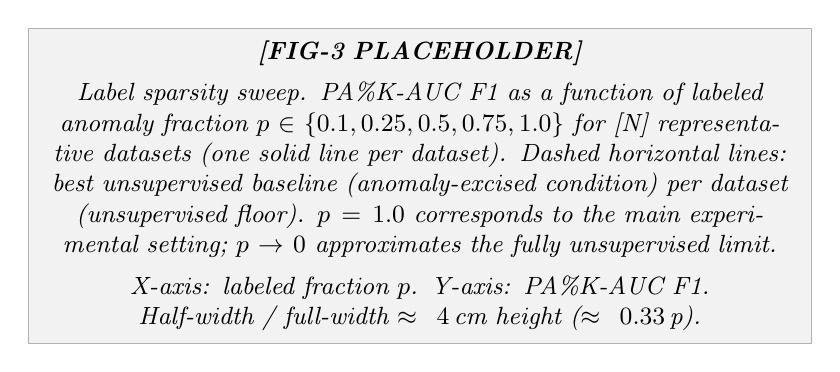
\begin{tikzpicture}
    % height = REGISTRY assumption (~4 cm = 0.33p)
    \node[draw=gray!60, fill=gray!10, minimum width=0.82\linewidth, minimum height=4.0cm,
          text width=0.78\linewidth, align=center, font=\small\itshape] (box) {%
      \textbf{[FIG-3 PLACEHOLDER]}\\[4pt]
      Label sparsity sweep.
      PA\%K-AUC F1 as a function of labeled anomaly fraction
      $p \in \{0.1, 0.25, 0.5, 0.75, 1.0\}$ for [N] representative datasets
      (one solid line per dataset).
      Dashed horizontal lines: best unsupervised baseline (anomaly-excised condition)
      per dataset (unsupervised floor).
      $p=1.0$ corresponds to the main experimental setting;
      $p \to 0$ approximates the fully unsupervised limit.\\[4pt]
      X-axis: labeled fraction $p$. Y-axis: PA\%K-AUC F1.
      Half-width / full-width $\approx 4$\,cm height ($\approx 0.33$\,p).
    };
  \end{tikzpicture}
  \caption{Label sparsity sweep. PA\%K-AUC F1 as a function of the labeled anomaly fraction
    $p \in \{0.1, 0.25, 0.5, 0.75, 1.0\}$ for [N] representative datasets (one line per
    dataset).
    Dashed horizontal lines indicate the performance of the best unsupervised baseline
    (anomaly-excised condition, main protocol) on the corresponding dataset, providing the
    unsupervised floor.
    $p = 1.0$ corresponds to the main experimental setting; $p \to 0$ approximates the fully
    unsupervised limit.}
  \label{fig:sparsity}
\end{figure}

Performance declines as $p$ decreases, [gradually\,/\,monotonically], % PH:NUM-027
retaining [competitive/partial] detection at $p = 0.25$ and approaching the best unsupervised
baseline as $p \to 0$, consistent with CSMAD reverting to its reconstruction-based mode at the
unsupervised floor.
% PH:TXT-003 | resolve [competitive/partial] and degradation-shape descriptor from Fig. 3

\subsection{Qualitative Analysis}
\label{sec:qualitative}

Figure~\ref{fig:decomp} decomposes the CSMAD anomaly score for representative windows from [N]
datasets into four aligned traces: raw input, reconstruction error, discrepancy, and the
thresholded combined score.
% PH:NUM-028 | number of datasets in Fig. 4

% ---- Figure 4: Qualitative score decomposition ----
\begin{figure}[tbp]
  \centering
  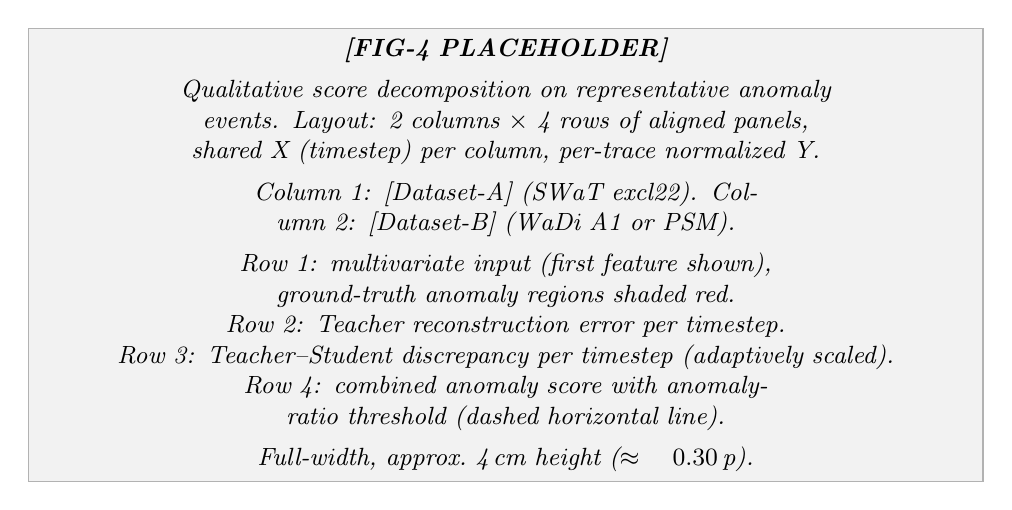
\begin{tikzpicture}
    % height = REGISTRY compression-ladder lower bound (3.5 cm; assumption 3.5-4 cm = 0.30p)
    \node[draw=gray!60, fill=gray!10, minimum width=\linewidth, minimum height=3.5cm,
          text width=0.92\linewidth, align=center, font=\small\itshape] (box) {%
      \textbf{[FIG-4 PLACEHOLDER]}\\[4pt]
      Qualitative score decomposition on representative anomaly events.
      Layout: 2 columns $\times$ 4 rows of aligned panels, shared X (timestep) per column,
      per-trace normalized Y.\\[4pt]
      Column 1: [Dataset-A] (SWaT excl22).
      Column 2: [Dataset-B] (WaDi A1 or PSM).\\[4pt]
      Row 1: multivariate input (first feature shown), ground-truth anomaly regions shaded red.\\
      Row 2: Teacher reconstruction error per timestep.\\
      Row 3: Teacher--Student discrepancy per timestep (adaptively scaled).\\
      Row 4: combined anomaly score with anomaly-ratio threshold (dashed horizontal line).\\[4pt]
      Full-width, approx.\ 4\,cm height ($\approx 0.30$\,p).
    };
  \end{tikzpicture}
  \caption{Qualitative score decomposition on representative anomaly events.
    Each column corresponds to one dataset ([Dataset-A], [Dataset-B]).
    Row~1: multivariate input (first feature shown) with ground-truth anomaly regions shaded in
    red.
    Row~2: Teacher reconstruction error per timestep.
    Row~3: Teacher--Student discrepancy per timestep (adaptively scaled).
    Row~4: combined anomaly score with the anomaly-ratio threshold (dashed horizontal line).
    The decomposition illustrates how the two score components respond differently to anomaly
    characteristics: reconstruction error captures deviations from the learned normal pattern
    regardless of event type, while discrepancy captures structural divergence amplified by the
    capacity gap and label-guided training.}
  \label{fig:decomp}
\end{figure}

The two components respond distinctly: reconstruction error rises wherever the input deviates from
learned normal patterns, while the discrepancy captures the additional divergence where the
Student's suppressed representation fails to replicate the Teacher.

%% PDF QA r1 MAJOR-8: keep this section's floats from drifting past the section end
\BodyFloatBarrier
